\section{Introduction}
\label{sec:intro}

\lightlipsum[1]

\begin{figure} [h]
	\begin{center}
	\begin{subfigure}[b]{0.32\textwidth}
		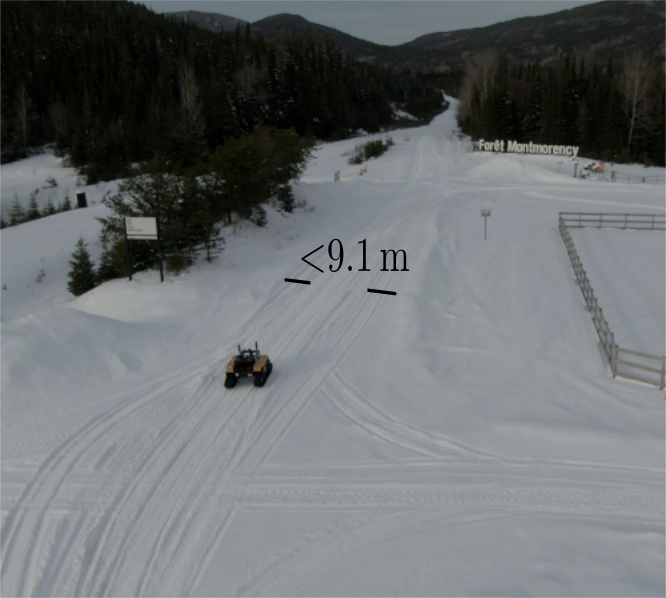
\includegraphics[width=\linewidth]{figs/intro/large_path_inkscape.pdf}
		\caption{A photo of a forest road.}
		\label{fig:large_path}
	\end{subfigure}%
	~
	\begin{subfigure} [b] {0.32\textwidth}
		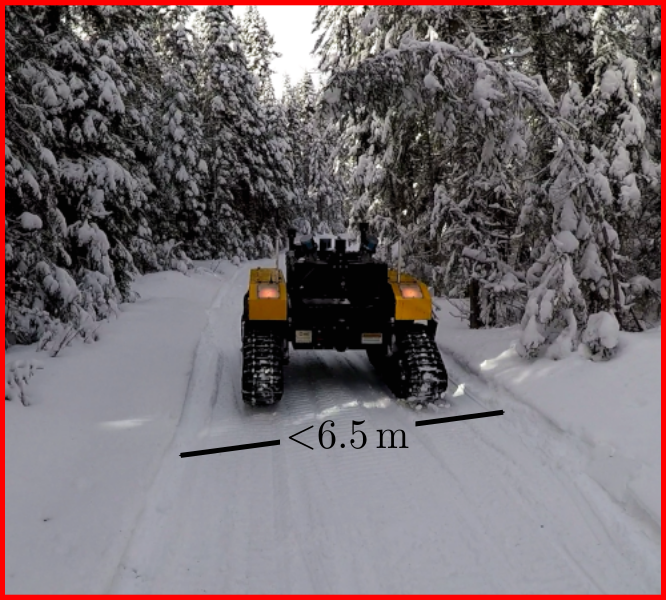
\includegraphics[width=\linewidth]{figs/intro/narrow_path_inkscape.pdf}
		\caption{A photo of a forest trail.}
		\label{fig:narrow_path}
	\end{subfigure}
	~~
	\begin{subfigure} [b] {0.32\textwidth}
		\includegraphics[width=\linewidth]{figs/intro/woods_inkscape.pdf}
		\caption{A photo of dense wood.}
		\label{fig:wood}
	\end{subfigure}
	\end{center}
	\caption{Our \ac{LTR} framework was designed to be used in subarctic off-road environments.
	Various paths can be driven on in such environments, namely forest roads and forest trails. 
	The main focus of this work is autonomous \ac{LTR} on forest trails, which have a maximum width of \SI{6.5}{m}.
	Our work does not cover deep woods navigation, in which our system would not be viable.}
	\label{fig:intro}
\end{figure}

\lightlipsum[1]
\lightlipsum[1]
\lightlipsum[1]

% Discuss lifelong learning